\chapter{Experimental Apparatus \label{sec:app}}

\section{Introduction}

The apparatus used for this paper is a combination of a large particle accelerator complex and a detector used to measure the results of particle collisions.
%r than how the term is normally used.  
Protons are accelerated and brought to a collision by the Large Hadron Collider (LHC)
located outside Geneva, Switzerland spanning the Swiss-French border. The protons are accelerated in smaller linear and cyclical accelerators before being injected
into the LHC. The protons are brought to a collision at four spots along the LHC. Surrounding one of these spots is the Compact Muon Solenoid (CMS) detector. The CMS
detector consists of multiple subsystems which work together to identify signatures of different types of particles.

\section{Large Hadron Collider \label{sec:LHC}}
A full description of the LHC can be found in~\cite{1748-0221-3-08-S08001}, a short summary is included here.
The LHC is a two-ring superconducting synchotron designed
to collide particles at high energy and high luminosity. It sits in a 26.7 km tunnel located 45-170m underneath the Swiss-French countryside outside of Geneva, Switzerland.
The LHC can create collisions with either protons or heavier ions. This leads to three possible operational modes, proton-proton, ion-ion, and proton-ion.
Only in proton-proton operational mode is there a possibility to discover HSCPs and it is the only mode discussed in this paper.

The LHC was designed to accelerate protons to an energy of seven TeV and collide them at a center of mass energy($\sqrt{s}$) of 
fourteen TeV with an instantaneous luminosity of $10^{34}cm^{-2}s^{-1}$. The protons are brought
to a collision at four points along the LHC beamline. Surrounding two of these interaction points sit the general purpose detectors of CMS and ATLAS. These detectors are 
meant to recieve the highest instantaneous luminosity the LHC can supply. The other interaction points are surrounded by the special purpose detectors LHCb and ALICE and
are designed to have instantaneous luminosities of $2\times10^{29}cm^{-2}s^{-1}$ and $10^{27}cm^{-2}s^{-1}$, respectively. This paper considers data collected by the
CMS detector.

The acceleration of protons to their final energy of 7 TeV is done in series of steps employing smaller accelerators located on the CERN campus. 
The protons originate in the linear accelerator Linac2 where they are passed through a series of synchotron accelerators, the Proton Synchotron Booster, the Proton Synchotron,
and the Super Proton Synchotron, with their energy raised to 1.4 GeV, 25 GeV, and 450 GeV, respectively. After passing through the Super Proton Synchotron the protons
are passed into the LHC. The LHC then accelerates the protons to their final design energy of 7 TeV.

The beams are designed to contain proton bunches spaced such that collisions at the interaction points occur every 25ns. 
%Running at the LHC thus far
%This time span sets the window of 
The LHC can hold a total of 2,808 bunches, in some places it is designed to have are gaps larger than 25ns between bunches to allow for dumping of the beam without harming the LHC.
Each 25ns time window is referred to as a bunch crossing window, whether there are proton bunches colliding in CMS or not.
Each collision between the proton bunches can
result in more than one proton-proton collision. This results in the the detectors around the LHC interaction points seeing numerous proton-proton collisions
overlayed on one another.
%The effect of this on the search for HSCPs is discussed in Section~\ref{sec:SystUnc}.

The commisioning of the LHC saw it run at a progression of lower energies building towards the design energy. In 2008 the LHC was run at
$\sqrt{s}=900$ GeV and for a short period at 2.36 TeV. Then after further work on the LHC, the energy was raised to 7 TeV for both 2010 and 2011 and then to 8 TeV in 2012.
This paper only covers the data collected at 7 and 8 TeV in 2011 and 2012. It is planned to raise the energy to its design goal of 14 TeV through additional work on the
LHC and the injector system.

Similarly, the instantaneous luminosity was ramped up during the commisioning phase. During the 2012 running, the machine ran with the proton bunches separated by 50ns.
The instantaneous luminosity often reached $7\times10^{33}cm^{-2}s^{-1}$. With 50ns spacing this means that the per bunch luminosity actually exceeded
the design value. It is planned to run with 25ns bunch spacing in future LHC running.

\section{Compact Muon Solenoid}

The CMS detector is built around one of the interaction points of the LHC. A full description of CMS be found in 
references~\cite{Chatrchyan:2008zzk, Bayatian:922757}.

CMS was designed to be a general purpose detector that would have sensitivity to a wide range of physics. This is important for a search for HSCP as the detector
is used in ways not typically done in most CMS analyses.
The central feature of CMS is a superconducting solenoid magnet with a 6m diameter and 13m length that provides a 3.8T magnetic field. The return field from the solenoid
is powerful enough to saturate 1.5m of iron, this allows for a strong magnetic field to be present outside of the solenoid.
CMS has a cylindrical shape with an onion like design where inner subdetectors are nested inside of outer ones. From inside out these subdetectors are an all silicon
tracker, an electromagnetic and hadronic calorimeter, the magnet, and finally the muon system. The various subdetectors and their role in identifying
SM particles can be seen in Figs~\ref{fig:CMSPart} and~\ref{fig:CMSSlice}.

CMS employs a right handed coordinate system with the x-axis pointing to the center of the LHC ring, the y-axis pointing vertically upward, and thus making the z-axis
be along the beam line pointing in the clockwise direction if looking at the LHC from above. The azimuthal angle, $\theta$, is defined relative to the z-axis. The variable
psuedorapidity, $\eta$, is defined as $\eta = -\ln{[\tan{(\theta/2)}]}$. The polar angle, $\phi$, is defined relative to the x-axis, meaning that vertically
upward (downward) has a $\phi$ value of $\pi/2$ ($-\pi/2$).

\begin{figure}
  \begin{center}
      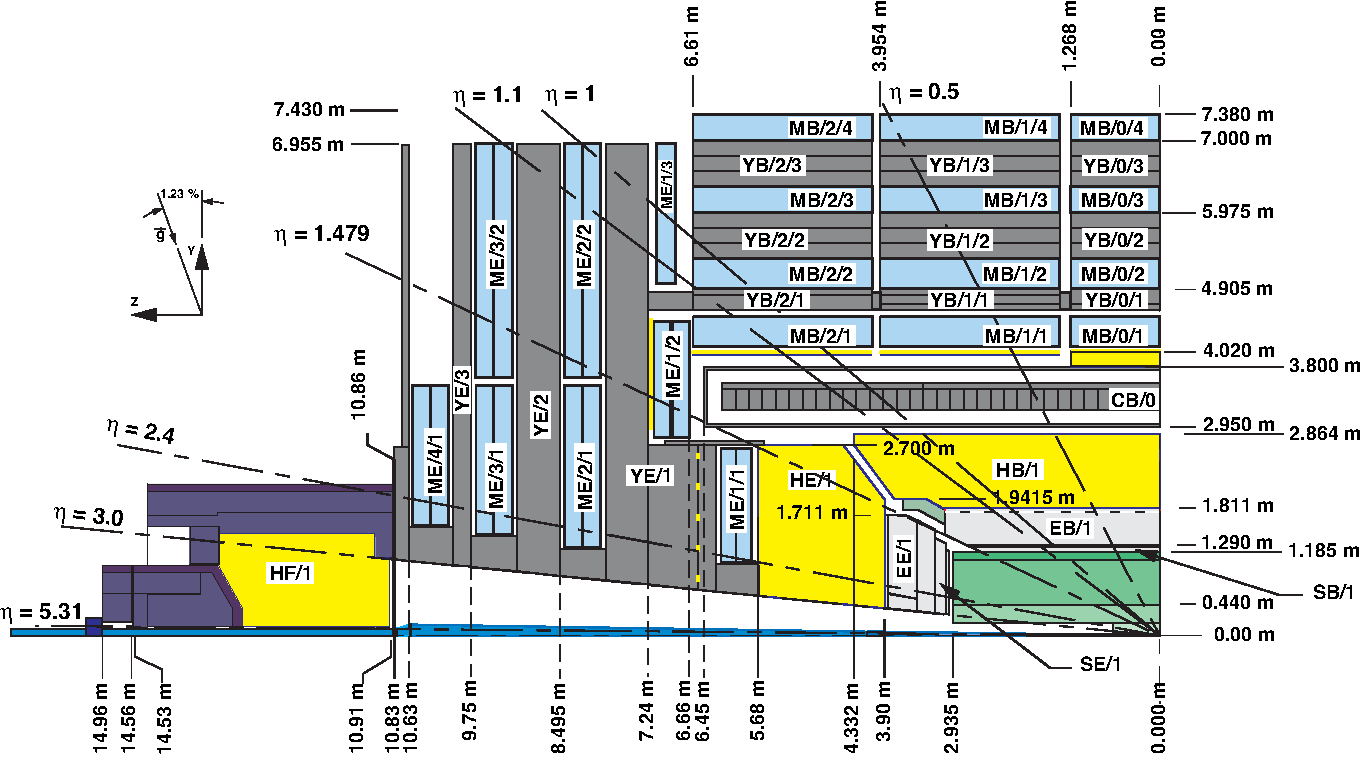
\includegraphics[clip=true, trim=0.0cm 0cm 3.0cm 0cm, width=0.9\textwidth]{figures/apparatus/CMS_LongView_noME42.pdf}
        \caption[Cross-section view of CMS detector]
        {Cross section of CMS detector. Inner silicon track bottom right in green, electromagnetic and hadronic calorimeter in light gray and yellow, respectively.
Muon detectors on the outside in blue.
         }
      \label{fig:CMSPart}
  \end{center}
\end{figure}

\begin{figure}
  \begin{center}
      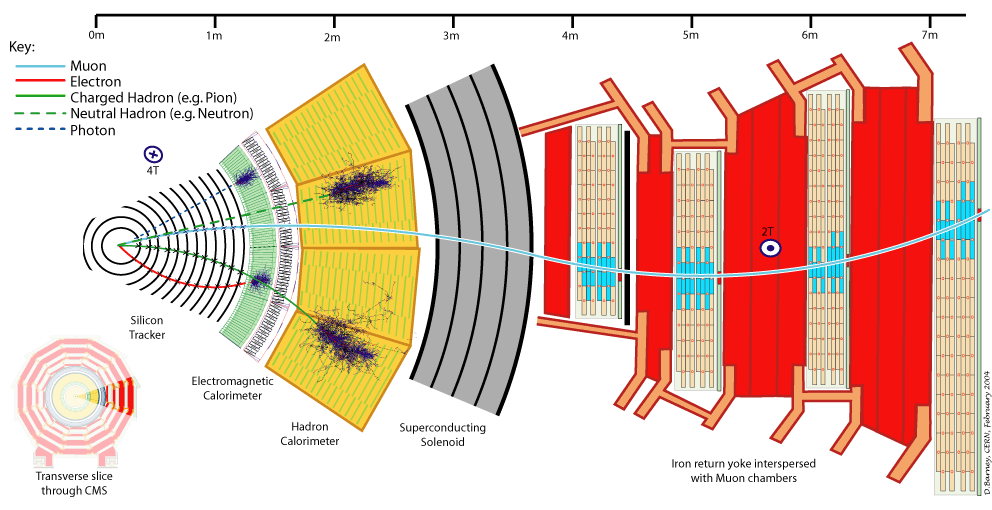
\includegraphics[clip=true, trim=0.0cm 0cm 3.0cm 0cm, width=\textwidth]{figures/apparatus/CMS_Slice.png}
        \caption{Expected interactions of SM particles as they propagate through CMS.
        }
      \label{fig:CMSSlice}
  \end{center}
\end{figure}

The possibility that a particle containing an HSCP can interact with the detector and change its charge
means that it may not look like any of the particles in Figure~\ref{fig:CMSSlice}. The particle
may be produced neutral and only gain charge as it passes through the calorimeter. The only record of its hits will be in the muon system giving the signature shown in
Figure~\ref{fig:CMSMuOnly}. In addition, the particle may be produced charged charged but then become neutral after interacting with CMS giving the signature shown in
Figure~\ref{fig:CMSTkOnly}. To discover HSCP with these exotic signatures it is necessary to conduct dedicated searches.
Searches of this type are presented in Chapter~\ref{sec:search}.



\begin{figure}
  \begin{center}
      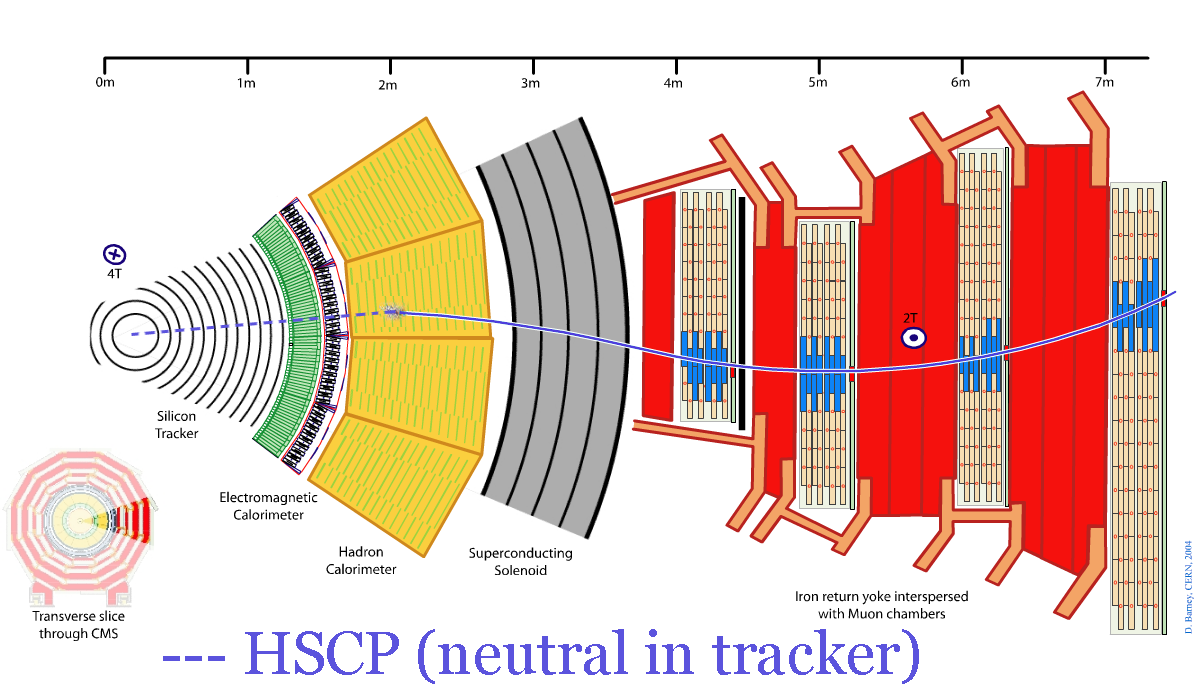
\includegraphics[clip=true, trim=0.0cm 0cm 3.0cm 0cm, width=0.9\textwidth]{figures/apparatus/ParticleInCMS_0009_Becoming_Charged}
      \caption[HSCP produced neutral and only becoming charged after interacting with the CMS detector.]
        {HSCP produced neutral and only becoming charged after interacting with the CMS detector.
	 }
      \label{fig:CMSMuOnly}
  \end{center}
\end{figure}

\begin{figure}
  \begin{center}
      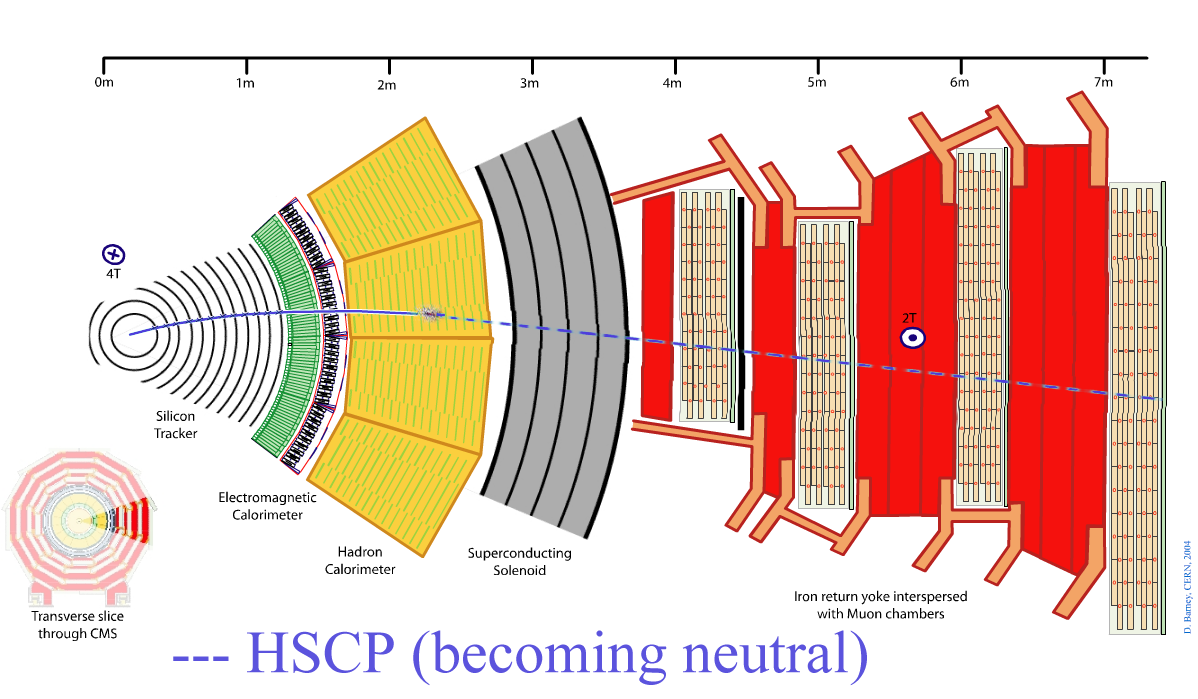
\includegraphics[clip=true, trim=0.0cm 0cm 3.0cm 0cm, width=0.9\textwidth]{figures/apparatus/ParticleInCMS_0000_HSCP-(becoming-neutral).png}
      \caption[HSCP produced charged and becoming neutral after interacting with the CMS detector.]
        {HSCP produced charged and only becoming neutral after interacting with the CMS detector.
         }
      \label{fig:CMSTkOnly}
  \end{center}
\end{figure}

\subsection{Subdetectors \label{sec:subsystems}}
The innermost part of CMS is an all silicon tracker. Closest to the interaction point are pixel detectors with three barrel layers and two endcap disks, totalling 1,440 modules. 
Outside of this are strip detectors with ten barrel layers and twelve endcap disks. It extends up to a psuedorapidity range of 2.5 with the resolution on track
$p_T$ being approxiamtely 1.5\% for a 100 GeV$/c$ particle at $|\eta| = 1.6$ and growing larger at high $|\eta|$ due to the decreased lever arm. Both the strips and the
pixels have an analog readout of the deposited charge with a maximum readout of roughly three times the charge expected to be deposited by a muon. Charge from
particles traversing the inner tracker is expected to be spread out among multiple modules in the same layer allowing the position of the particle to be calculated
more precisely then simply the center of the module. The charge sharing also allows the possibility to identify hits where two particles have overlapped.

Outside of the inner tracker is the calorimeter. The purpose of the calorimeter is to measure the energy of particles and aid in their identification by stopping
particles at different points in the calorimeter.  The calorimeter is split into an inner electromagnetic calorimeter (ECAL) and an outer hadronic calorimeter (HCAL). 
The ECAL is made of 75,848 lead tungstate ($PBWO_4$) crystals split between the barrel and endcap. As particles lose energy in the ECAL
the crystals emit scintillation light which is collected by photodetectors. The HCAL consists of plates of brass absorbers interleaved with scintillator
detectors.  Electrons and photons are likely to stop in the ECAL where they deposit all of their energies. Hadrons, electrically charged or neutral, will
deposit some energy in the ECAL but will deposit most in the HCAL where they are very likely to come to a rest. Muons will deposit of the order of two GeV of energy in
the calorimeter and are generally the only charged SM particles that are able to exit the calorimeter.

The outermost part of the detector is the muon system which is split into three parts, Cathode Strip Chambers(CSC), Drift Tubes(DT), and Resistive Plate Chambers(RPC).
The CSC cover the forward part of the detector with $|\eta|>0.9$ while the DT and the RPC cover the barrel portion extending up to $|\eta|$ of 1.2 and 1.6, respectively.
The muon system is comprised of four stations of chambers with the lead for the magnet return yoke located between the stations. The magnet return yoke provides a magnetic field
in the muon system.

CSC chambers have a trapezoidal shape with six layers of cathode strips and anode wires arranged in a nearly orthogonal pattern. 
The strips run radially away from the beam line and measure the $\phi$ of hits while the wires measure the radial position of hits. Charge collected on the wires
is passed to a constant fraction discriminator which outputs a 40ns pulse. The pulse is sampled every 25ns and this sampling is readout. The amount of charge on the strips
is readout every 50ns. The charge is used offline to get a more precise estimate of the position and time of the hit.
The CSCs are layed out with four stations with increasing $z$ from the interaction point and rings of increasing radial distance from the beam line.

DT chambers have two or three superlayers which themselves are composed of four layers of drift cells which are staggered by half a cell. All of the DT chambers have
two superlayers oriented parallel to the beam line, these superlayers measure the position of particles in the $r-\phi$ plane.
The three inner stations additionally have a superlayer running perpendicular to the beamline to measure the position of particles in the $r-z$ plane.

RPC chambers are gaseous parallel plate detectors that can provide a time resolution of 2ns, which is much smaller than the design LHC bunch spacing of 25ns allowing for
a very high efficiency to correctly tag hits with the correct event. The spatial resolution is sufficient to be able to associate RPC hits with hits
from the other muon subdetectors.

\subsection{Computing \label{sec:computing}}
The rate of proton-proton collisions inside of CMS is too large for all of them to be readout and stored offline. To deal with this CMS employs a two level trigger
that selects interesting events online. The level one (L1) trigger must reduce the rate of events readout to less than 100 kHz in less than 3$\mu s$
requiring a completely firmware based approach. Events are selected by a variety of algorithms but most of them look for a high momentum track in the muon
system, large amount of energy in the ECAL or HCAL, or a combination of these. Signals from these systems trigger the readout of the rest of detector through
the data acquisition system. As the LHC was designed to operate with 25 ns bunch spacing many of the subsystems, the tracker especially, only readout
the data in the 25ns window associated with the event. This means that triggers that pre or post-fire will not contain much of the data from the event.
This can be issue for HSCP that are travelling so slowly that they reach the muon system in the time window associated with the next bunch crossing window.
However, a special configuration of the RPC trigger exploits the fact that current running of the LHC has been done with at least 50ns spacing

All hits in the RPC are sent to the trigger electronics twice, once for the bunch crossing window they are associated with and also for the one proceeding it.
From there the trigger electronics treat the advanced RPC hits in the same manner as they do all other hits. 
This allows the RPCs to trigger the readout of the event preceeding the arrival of the particle in the RPCs.
This means that HSCP which arrive to the muon system up to 37.5ns after
a muon is expected could still trigger the readout of the correct data in the rest of the detector.
% corresponding with the bunch crossing window it was created in.

%Despite the RPC signaling to readout two events only one will ever be actually collected as readout of consecutive events is forbidden by the DAQ. 
To ensure collision muons still maintain the correct behavior, accept signals sent for the bunch crossing window immediately
preceeding a bunch crossing window with protons passing through CMS are rejected. 
So signals from collision muons will attempt to pretrigger but this will be vetoed and the following event will be correctly readout.
%A schema illustrating this behavior is shown in~\ref{fig:RPC_HSCP}. 
This configuration is only possible  when proton collsions are spaced by at least 50ns so that accept signals from successive 25ns
bunch crossing windows can be unambiguously classified.

%\begin{figure}
% \begin{center}
%  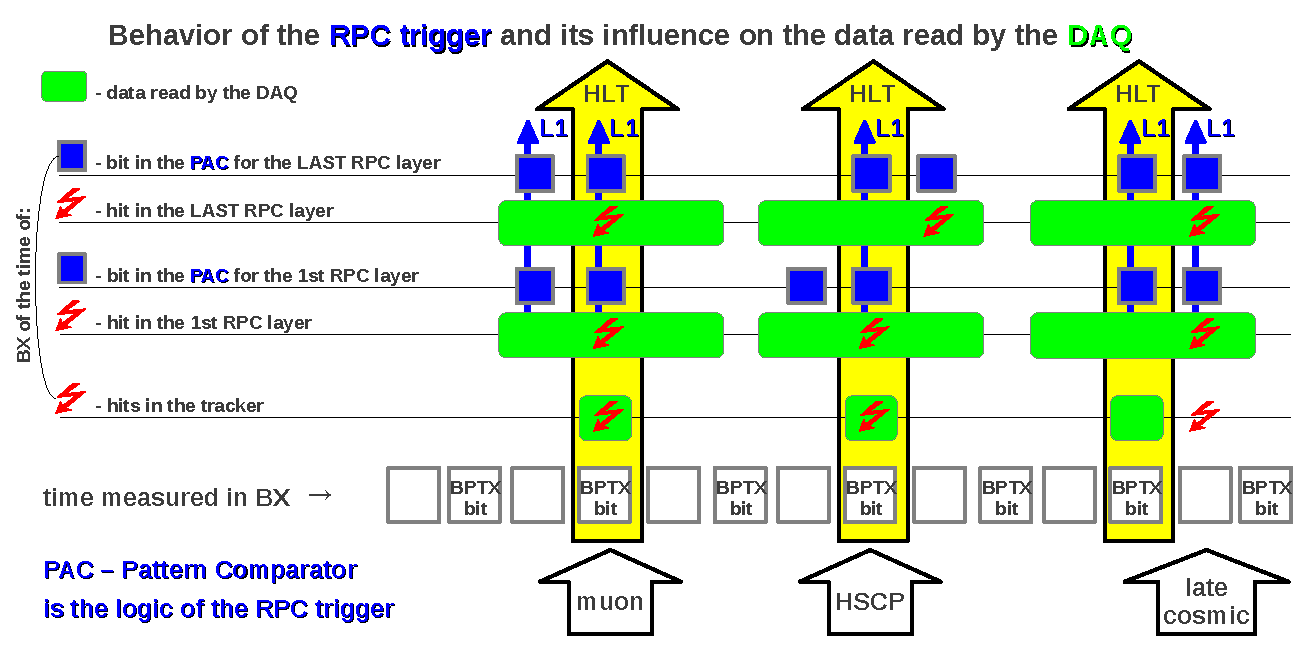
\includegraphics[clip=true, trim=0.0cm 0cm 0.0cm 0cm, width=1.0\linewidth]{figures/RPC_HSCP}
% \end{center}
% \caption{Way too long... Schema of a~temporal behavior of the RPC trigger and
%its influence on the data read by the data acquisition system.
%Time measured in BX quanta goes from left to right.
%The results of appearance
%of three (separate in time) objects of different type is shown:
%pp collision
%muon, HSCP which is delayed by one BX at the exit from the muon system and
%outward going cosmic muon delayed by one BX with respect to muons
%from pp collision.
%Each hit (read bolts) in the RPC is advanced by one BX and duplicated
%(blue squares) in the PAC
%(Pattern Comparator, chip in which main part of the RPC trigger
%logic is implemented). Only first and last RPC layers are shown.
%A~coincidence (pattern) of bits in the PAC in the same BX gives L1 trigger
%(blue arrows). But to obtain the HLT trigger a coincidence of
%the RPC L1 trigger with BPTX bit is required (yellow arrows).
%DAQ reads tracker data from HLT selected BX and RPC data from adjacent BXs
%(green rectangles). Both pp mouns and (not too slow)
%HSCPs give HLT trigger.
%Outward cosmic muons, which are late by one BX, also give HLT trigger
%(rightmost yellow arrow), but its tracker hits are not selected.
%Such cosmic muons will not become global muons.}
%   \label{fig:RPC_HSCP}
%\end{figure}

The next step in the trigger is the High Level Trigger (HLT) which must reduce the number of events to a few hundred Hz on the order of a second. The HLT
is software based and there are a wide variety of algorithms used to identify interesting events and store them for offline analysis. The HLT is split into two different
phases, Level 2 (L2), and Level 3 (L3). The L2 step is mostly concerned with confirming the L1 decision and reducing the rate so that higher level objects
can be built within the time restrictions. The L3 step builds these objects, often reconstructing tracks of particles in the inner tracker and matching them
to objects in other parts of the detector, and then applies requirements on the objects selecting which events to pass for storage at computers located at CERN
and throughout the world.

CMS maintains a software, CMSSW, which is responsible for taking the raw data readout from CMS and reconstructing what was happening in the event.
This includes applying calibration constants, finding tracks, and indentifying particles.
%attempts to reconstruct the particles in the event, identify them as one of the long-lived SM particles, give 
%a multitude of information about the particle, and apply any necessary calibration constants. 
%The code also calculates event level quantities such as the total momentum of all the particles in the event. 
After this reconstruction, the data size is at the scale of petabytes which is too large for offline analyzers to run over frequently. 
To deal with this copies of the data are produced dropping lower level quantities and selecting only events that a particular analysis is interested in studying.

CMSSW is also tasked with simulating how particles, coming from both SM processes and new physics, would interact with the detector so that this can be used to
compare against data. Two steps are performed before the simulation has the same format as data readout from the detector, at that
point it follows the same chain as data. The first step is the simulation of the proton-proton collision
and the particles that are created from it, the detector is not used at all in this step. The next step is the simulation of the interaction of these particles with the detector
and the behavior of the detector electronics, including the L1 trigger. After this point, the simulation is handled the same as data.